% Options for packages loaded elsewhere
\PassOptionsToPackage{unicode}{hyperref}
\PassOptionsToPackage{hyphens}{url}
%
\documentclass[
]{article}
\usepackage{amsmath,amssymb}
\usepackage{iftex}
\ifPDFTeX
  \usepackage[T1]{fontenc}
  \usepackage[utf8]{inputenc}
  \usepackage{textcomp} % provide euro and other symbols
\else % if luatex or xetex
  \usepackage{unicode-math} % this also loads fontspec
  \defaultfontfeatures{Scale=MatchLowercase}
  \defaultfontfeatures[\rmfamily]{Ligatures=TeX,Scale=1}
\fi
\usepackage{lmodern}
\ifPDFTeX\else
  % xetex/luatex font selection
\fi
% Use upquote if available, for straight quotes in verbatim environments
\IfFileExists{upquote.sty}{\usepackage{upquote}}{}
\IfFileExists{microtype.sty}{% use microtype if available
  \usepackage[]{microtype}
  \UseMicrotypeSet[protrusion]{basicmath} % disable protrusion for tt fonts
}{}
\makeatletter
\@ifundefined{KOMAClassName}{% if non-KOMA class
  \IfFileExists{parskip.sty}{%
    \usepackage{parskip}
  }{% else
    \setlength{\parindent}{0pt}
    \setlength{\parskip}{6pt plus 2pt minus 1pt}}
}{% if KOMA class
  \KOMAoptions{parskip=half}}
\makeatother
\usepackage{xcolor}
\usepackage[margin=1in]{geometry}
\usepackage{color}
\usepackage{fancyvrb}
\newcommand{\VerbBar}{|}
\newcommand{\VERB}{\Verb[commandchars=\\\{\}]}
\DefineVerbatimEnvironment{Highlighting}{Verbatim}{commandchars=\\\{\}}
% Add ',fontsize=\small' for more characters per line
\usepackage{framed}
\definecolor{shadecolor}{RGB}{248,248,248}
\newenvironment{Shaded}{\begin{snugshade}}{\end{snugshade}}
\newcommand{\AlertTok}[1]{\textcolor[rgb]{0.94,0.16,0.16}{#1}}
\newcommand{\AnnotationTok}[1]{\textcolor[rgb]{0.56,0.35,0.01}{\textbf{\textit{#1}}}}
\newcommand{\AttributeTok}[1]{\textcolor[rgb]{0.13,0.29,0.53}{#1}}
\newcommand{\BaseNTok}[1]{\textcolor[rgb]{0.00,0.00,0.81}{#1}}
\newcommand{\BuiltInTok}[1]{#1}
\newcommand{\CharTok}[1]{\textcolor[rgb]{0.31,0.60,0.02}{#1}}
\newcommand{\CommentTok}[1]{\textcolor[rgb]{0.56,0.35,0.01}{\textit{#1}}}
\newcommand{\CommentVarTok}[1]{\textcolor[rgb]{0.56,0.35,0.01}{\textbf{\textit{#1}}}}
\newcommand{\ConstantTok}[1]{\textcolor[rgb]{0.56,0.35,0.01}{#1}}
\newcommand{\ControlFlowTok}[1]{\textcolor[rgb]{0.13,0.29,0.53}{\textbf{#1}}}
\newcommand{\DataTypeTok}[1]{\textcolor[rgb]{0.13,0.29,0.53}{#1}}
\newcommand{\DecValTok}[1]{\textcolor[rgb]{0.00,0.00,0.81}{#1}}
\newcommand{\DocumentationTok}[1]{\textcolor[rgb]{0.56,0.35,0.01}{\textbf{\textit{#1}}}}
\newcommand{\ErrorTok}[1]{\textcolor[rgb]{0.64,0.00,0.00}{\textbf{#1}}}
\newcommand{\ExtensionTok}[1]{#1}
\newcommand{\FloatTok}[1]{\textcolor[rgb]{0.00,0.00,0.81}{#1}}
\newcommand{\FunctionTok}[1]{\textcolor[rgb]{0.13,0.29,0.53}{\textbf{#1}}}
\newcommand{\ImportTok}[1]{#1}
\newcommand{\InformationTok}[1]{\textcolor[rgb]{0.56,0.35,0.01}{\textbf{\textit{#1}}}}
\newcommand{\KeywordTok}[1]{\textcolor[rgb]{0.13,0.29,0.53}{\textbf{#1}}}
\newcommand{\NormalTok}[1]{#1}
\newcommand{\OperatorTok}[1]{\textcolor[rgb]{0.81,0.36,0.00}{\textbf{#1}}}
\newcommand{\OtherTok}[1]{\textcolor[rgb]{0.56,0.35,0.01}{#1}}
\newcommand{\PreprocessorTok}[1]{\textcolor[rgb]{0.56,0.35,0.01}{\textit{#1}}}
\newcommand{\RegionMarkerTok}[1]{#1}
\newcommand{\SpecialCharTok}[1]{\textcolor[rgb]{0.81,0.36,0.00}{\textbf{#1}}}
\newcommand{\SpecialStringTok}[1]{\textcolor[rgb]{0.31,0.60,0.02}{#1}}
\newcommand{\StringTok}[1]{\textcolor[rgb]{0.31,0.60,0.02}{#1}}
\newcommand{\VariableTok}[1]{\textcolor[rgb]{0.00,0.00,0.00}{#1}}
\newcommand{\VerbatimStringTok}[1]{\textcolor[rgb]{0.31,0.60,0.02}{#1}}
\newcommand{\WarningTok}[1]{\textcolor[rgb]{0.56,0.35,0.01}{\textbf{\textit{#1}}}}
\usepackage{graphicx}
\makeatletter
\def\maxwidth{\ifdim\Gin@nat@width>\linewidth\linewidth\else\Gin@nat@width\fi}
\def\maxheight{\ifdim\Gin@nat@height>\textheight\textheight\else\Gin@nat@height\fi}
\makeatother
% Scale images if necessary, so that they will not overflow the page
% margins by default, and it is still possible to overwrite the defaults
% using explicit options in \includegraphics[width, height, ...]{}
\setkeys{Gin}{width=\maxwidth,height=\maxheight,keepaspectratio}
% Set default figure placement to htbp
\makeatletter
\def\fps@figure{htbp}
\makeatother
\setlength{\emergencystretch}{3em} % prevent overfull lines
\providecommand{\tightlist}{%
  \setlength{\itemsep}{0pt}\setlength{\parskip}{0pt}}
\setcounter{secnumdepth}{-\maxdimen} % remove section numbering
\ifLuaTeX
  \usepackage{selnolig}  % disable illegal ligatures
\fi
\IfFileExists{bookmark.sty}{\usepackage{bookmark}}{\usepackage{hyperref}}
\IfFileExists{xurl.sty}{\usepackage{xurl}}{} % add URL line breaks if available
\urlstyle{same}
\hypersetup{
  pdftitle={STAT 437 HW 3},
  hidelinks,
  pdfcreator={LaTeX via pandoc}}

\title{STAT 437 HW 3}
\author{}
\date{\vspace{-2.5em}2023-03-05}

\begin{document}
\maketitle

\textbf{NOTE}: Homework questions and instructions have been
\emph{italicized} for clarity.

\hypertarget{conceptual-exercises}{%
\section{Conceptual exercises}\label{conceptual-exercises}}

\noindent \textbf{1.} \emph{Consider the K-means clustering
methodology.}

\textbf{1.1)} \emph{Give a few examples of dissimilarity measures that
can be used to measure how dissimilar two observations are. What is the
main disadvantage of the squared Euclidean distance as a dissimilarity
measure?}

A few measures of similarity are the euclidean distance, the manhattan
distance, and the correlation distance.

The main disadvantage of the squared Euclidean distance is that it is
sensitive to outliers. Large distances will have an outsized influence
on the results.

\textbf{1.2)} \emph{Is it true that standardization of data should be
done when features are measured on very different scales? Is it true
that employing more features gives more accurate clustering results? Is
it true that employing standardized observations gives more accurate
clustering results than employing non-standardized ones? Explain each of
your answers.}

Standardization of data should be done when features are measured on
different scales. This ensures that that features don't have an outsized
impact because of their units.

Employing more features does not necessarily give more accurate
clustering results. This is related to the curse of dimensionality - if
you employ more features, you must have many more observations.

Employing standardized observations generally will improve clustering
results for the same reason mentioned above - it ensures that features
are weighted equally. If the units of all features are already the same,
then it is not necessary.

\textbf{1.3)} \emph{Take \(K=2\). Provide the loss function that K-means
clustering tries to minimize. You need to provide the definition and
meaning of each term that appears in the loss function.}

W(C) = \(\Sigma_1 d^2(x_i, x\bar_1) + \Sigma_2 d^2(x_i,x\bar_2)\)

W(C) is the loss of the mapping C

The first summand is the variance within that cluster - that is, the sum
of the euclidean distances between each point and the sample mean of
that cluster.

The second summand is the same for the second cluster.

\textbf{1.4)} \emph{What is the ``centroid'' for a cluster? Is the
algorithm, Algorithm 10.1 on page 388 of the Text (which is also
provided in the lecture slides), guaranteed to converge to the global
minimum of the loss function? Why or why not? What does the argument
\texttt{nstart} refer to in the command \texttt{kmeans}? Why is
\texttt{nstart} suggested to take a relatively large value? Why do you
need to set a random seed by \texttt{set.seed()} before you apply
\texttt{kmeans}?}

The centroid of the cluster is the coordinate associated with the mean
values among observations in the cluster of the p features in the data.
It is representative of the center of that cluster. The algorithm is not
guaranteed to converge to a global minimum. It may converge to a local
minimum at which point the cluster assignments stop changing, but that
local minimum may not match the global minimum. This is because

\textbf{1.5)} \emph{Suppose there are 2 underlying clusters but you set
the number of clusters to be different than \(2\) and apply
\texttt{kmeans}, will you have good clustering results? Why or why not?}

The cluster results will not never be accurate if the number of clusters
is set to be different than the true number of underlying clusters. If
K=2, then the best case scenario is that one of the clusters will be
entirely identified and the other will be split into two. This could
still be informative for data exploration.

\textbf{1.6)} \emph{Is the true number \(K_0\) of clusters in data
known? When using the command \texttt{clusGap} to estimate \(K_0\), what
does its argument \texttt{B} refer to?}

The true number of clusters in data is generally unknown. B is the
number of samples (resampled with replacement, i.e.~`bootstrap' samples)
that the clusGap function iwll use to estimate the true number of
clusters.

\noindent \textbf{2.} \emph{Consider hierarchical clustering.}

\_2.1)\_\_ \emph{What are some advantages of hierarchical clustering
over K-means clustering? What is the relationship between the
dissimilarity between two clusters and the height of these clusters in
the dendrogram that represents a bottom-up tree?}

Hierarchical clustering does not require that the number of the clusters
is specified and the resultant clusters don't depend on the
configuration of initially chosen clusters as in kmeans.

The height represents the dissimilarity between clusters at which point
they are fused.

\textbf{2.2)} \emph{Explain what it means by saying that ``the clusters
obtained at different heights from a dendrogram are nested''. If a data
set has two underlying clustering structures that can be obtained by two
different criteria, will these two sets of clusters necessarily be
nested? Explain your answer.}

The bottom-up approach of hierarchical clustering involves sequentially
joining clusters together. A cluster higher up in the tree consists of a
previous set of clusters that have been joined, so those clusters are
nested in the higher cluster. Hiearchical clustering will produce nested
clusters, but that nesting structure may not necessarily be
representative of the underlying structure. Hiearchical clustering does
not work well if the clusters are mutually exclusive.

\textbf{2.3)} \emph{Why is the distance based on Pearson's sample
correlation not effected by the magnitude of observations in terms of
Euclidean distance? What is the definition of average linkage? Why are
average linkage and complete linkage preferred than single linkage in
practice?}

Pearsons sample correlation is calculated using standardized values,
which removes the influence of magnitude.

Linkage is a measure of inter-cluster dissimilarity. Average linkage
computes the average of all dissimilarities between the observations of
two clusters. Single linkage is not preferred because of its tendency to
produce long, trailing clusters by adding a single observation to the
cluster each time.

\textbf{2.4)} \emph{What does the command \texttt{scale} do? Does
\texttt{scale} apply row-wise or column-wise? When \texttt{scale} is
applied to a variable, what will happen to the observations of the
variable?}

Scale is used to standardize columns - i.e.~it is applied column-wise.
The observations of a feature that scale is applied to first have the
feature's mean subtracted from them then are divided by the features
standard deviation. This centers and scales the observations -
i.e.~standardizes them.

\textbf{2.5)} \emph{What is \texttt{hclust\$height}? How do you find the
height at which to cut a dendrogram in order to obtain \(5\) clusters?}

hclust\$height is a set of heights that are equal to the dissimilarity
measure at each stage of agglomeration. To find the height at which to
cut the dendrogram to obtain 5 clusters one would take the 4th to last
value in the height.

\textbf{2.6)} \emph{When creating a dendrogram, what are some advantages
of the command \texttt{ggdendrogram\{ggdendro\}} over the R base command
\texttt{plot}?}

ggdendrogram creates cleaner visualizations of the dendrogram than the
base command. This includes advantages in label presentation and
coloring by cluster.

\hypertarget{applied-exercises}{%
\section{Applied exercises}\label{applied-exercises}}

\noindent \textbf{3.} \emph{Please refer to the NYC flight data
\texttt{nycflights13} tfhat has been discussed in the lecture notes and
whose manual can be found at
\url{https://cran.r-project.org/web/packages/nycflights13/index.html}.
We will use \texttt{flights}, a tibble from \texttt{nycflights13}.}

\begin{Shaded}
\begin{Highlighting}[]
\FunctionTok{library}\NormalTok{(nycflights13)}
\FunctionTok{library}\NormalTok{(tidyverse)}
\end{Highlighting}
\end{Shaded}

\begin{verbatim}
## -- Attaching core tidyverse packages ------------------------ tidyverse 2.0.0 --
## v dplyr     1.1.3     v readr     2.1.4
## v forcats   1.0.0     v stringr   1.5.0
## v ggplot2   3.4.3     v tibble    3.2.1
## v lubridate 1.9.2     v tidyr     1.3.0
## v purrr     1.0.2     
## -- Conflicts ------------------------------------------ tidyverse_conflicts() --
## x dplyr::filter() masks stats::filter()
## x dplyr::lag()    masks stats::lag()
## i Use the conflicted package (<http://conflicted.r-lib.org/>) to force all conflicts to become errors
\end{verbatim}

\emph{Select from \texttt{flights} observations that are for 3
\texttt{carrier} ``UA'', ``AA'' or ``DL'', for \texttt{month} 7 and 2,
and for 4 features \texttt{dep\_delay}, \texttt{arr\_delay},
\texttt{distance} and \texttt{air\_time}. Let us try to see if we can
use the 4 features to identify if an observation belongs a specific
carrier or a specific month. The following tasks and questions are based
on the extracted observations. Note that you need to remove
\texttt{na}'s from the extracted observations.}

\begin{Shaded}
\begin{Highlighting}[]
\NormalTok{flights.df }\OtherTok{\textless{}{-}}\NormalTok{ flights }\SpecialCharTok{\%\textgreater{}\%}
    \FunctionTok{select}\NormalTok{(carrier, month, dep\_delay, arr\_delay, distance, air\_time) }\SpecialCharTok{\%\textgreater{}\%}
    \FunctionTok{filter}\NormalTok{(carrier }\SpecialCharTok{\%in\%} \FunctionTok{c}\NormalTok{(}\StringTok{"UA"}\NormalTok{, }\StringTok{"AA"}\NormalTok{, }\StringTok{"DL"}\NormalTok{), month }\SpecialCharTok{\%in\%} \FunctionTok{c}\NormalTok{(}\DecValTok{7}\NormalTok{,}
        \DecValTok{2}\NormalTok{)) }\SpecialCharTok{\%\textgreater{}\%}
    \FunctionTok{na.omit}\NormalTok{()}

\NormalTok{flights.df}\SpecialCharTok{$}\NormalTok{carrier }\OtherTok{\textless{}{-}} \FunctionTok{as.factor}\NormalTok{(flights.df}\SpecialCharTok{$}\NormalTok{carrier)}
\NormalTok{flights.df}\SpecialCharTok{$}\NormalTok{month }\OtherTok{\textless{}{-}} \FunctionTok{as.factor}\NormalTok{(flights.df}\SpecialCharTok{$}\NormalTok{month)}
\end{Highlighting}
\end{Shaded}

\textbf{3.1)} \emph{Apply K-means with \(K=2\) and \(3\) respectively
but all with \texttt{set.seed(1)} and \texttt{nstart=20}. For \(K=3\),
provide visualization of the clustering results based on true clusters
given by \texttt{carrier}, whereas for \(K=2\), provide visualization of
the clustering results based on true clusters given by \texttt{month}.
Summarize your findings based on the clustering results. You can use the
same visualization scheme that is provided by Example 2 in
``LectureNotes3\_notes.pdf''. Try visualization based on different sets
of 2 features if your visualization has overlayed points.set.seed(1)}

\textbf{Perform Clustering}

\begin{Shaded}
\begin{Highlighting}[]
\FunctionTok{set.seed}\NormalTok{(}\DecValTok{1}\NormalTok{)}

\NormalTok{km.clus}\FloatTok{.2} \OtherTok{\textless{}{-}} \FunctionTok{kmeans}\NormalTok{(flights.df[}\DecValTok{3}\SpecialCharTok{:}\DecValTok{6}\NormalTok{], }\DecValTok{2}\NormalTok{, }\AttributeTok{nstart =} \DecValTok{20}\NormalTok{)}
\NormalTok{km.clus}\FloatTok{.3} \OtherTok{\textless{}{-}} \FunctionTok{kmeans}\NormalTok{(flights.df[}\DecValTok{3}\SpecialCharTok{:}\DecValTok{6}\NormalTok{], }\DecValTok{3}\NormalTok{, }\AttributeTok{nstart =} \DecValTok{20}\NormalTok{)}

\NormalTok{flights.df}\SpecialCharTok{$}\NormalTok{kmclus2 }\OtherTok{\textless{}{-}} \FunctionTok{factor}\NormalTok{(km.clus}\FloatTok{.2}\SpecialCharTok{$}\NormalTok{cluster)}
\NormalTok{flights.df}\SpecialCharTok{$}\NormalTok{kmclus3 }\OtherTok{\textless{}{-}} \FunctionTok{factor}\NormalTok{(km.clus}\FloatTok{.3}\SpecialCharTok{$}\NormalTok{cluster)}
\end{Highlighting}
\end{Shaded}

\textbf{K = 2 Visualization}

Attempting to cluster the observations to to identify the month in which
they occurred did not yield useful results. The plots do not show a
trend indicating that the clustering was successful and the confusion
matrix confirms this. Around half of the observations were clustered
wrong which is not pretty than the trivial solution of flipping a coin
to assign labels.

\begin{Shaded}
\begin{Highlighting}[]
\CommentTok{\# k = 2}
\FunctionTok{ggplot}\NormalTok{(flights.df) }\SpecialCharTok{+} \FunctionTok{geom\_point}\NormalTok{(}\FunctionTok{aes}\NormalTok{(dep\_delay, distance, }\AttributeTok{color =}\NormalTok{ kmclus2,}
    \AttributeTok{shape =}\NormalTok{ month)) }\SpecialCharTok{+} \FunctionTok{labs}\NormalTok{(}\AttributeTok{x =} \StringTok{"Departure Delay"}\NormalTok{, }\AttributeTok{y =} \StringTok{"Distance"}\NormalTok{,}
    \AttributeTok{title =} \StringTok{"K = 2"}\NormalTok{, }\AttributeTok{subtitle =} \StringTok{"Departure Delay vs. Distance"}\NormalTok{) }\SpecialCharTok{+}
    \FunctionTok{theme\_bw}\NormalTok{()}
\end{Highlighting}
\end{Shaded}

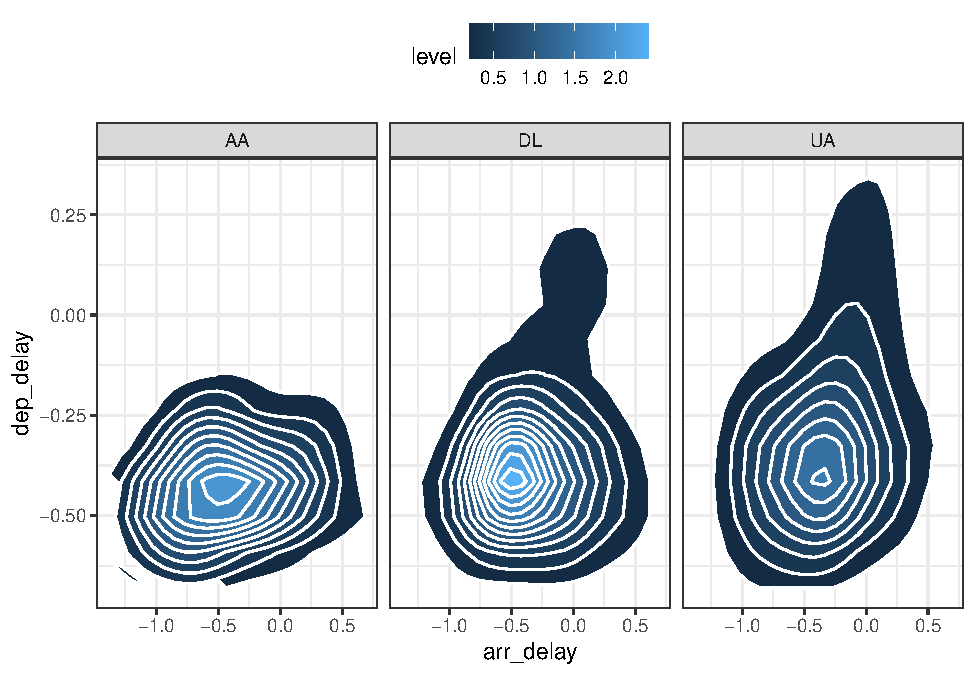
\includegraphics{stat437_HW3_files/figure-latex/unnamed-chunk-5-1.pdf}

\begin{Shaded}
\begin{Highlighting}[]
\FunctionTok{ggplot}\NormalTok{(flights.df) }\SpecialCharTok{+} \FunctionTok{geom\_point}\NormalTok{(}\FunctionTok{aes}\NormalTok{(arr\_delay, air\_time, }\AttributeTok{color =}\NormalTok{ kmclus2,}
    \AttributeTok{shape =}\NormalTok{ month)) }\SpecialCharTok{+} \FunctionTok{labs}\NormalTok{(}\AttributeTok{x =} \StringTok{"Arrival Delay"}\NormalTok{, }\AttributeTok{y =} \StringTok{"Air Time"}\NormalTok{,}
    \AttributeTok{title =} \StringTok{"K = 2"}\NormalTok{, }\AttributeTok{subtitle =} \StringTok{"Arrival Delay vs. Air Time"}\NormalTok{) }\SpecialCharTok{+}
    \FunctionTok{theme\_bw}\NormalTok{()}
\end{Highlighting}
\end{Shaded}

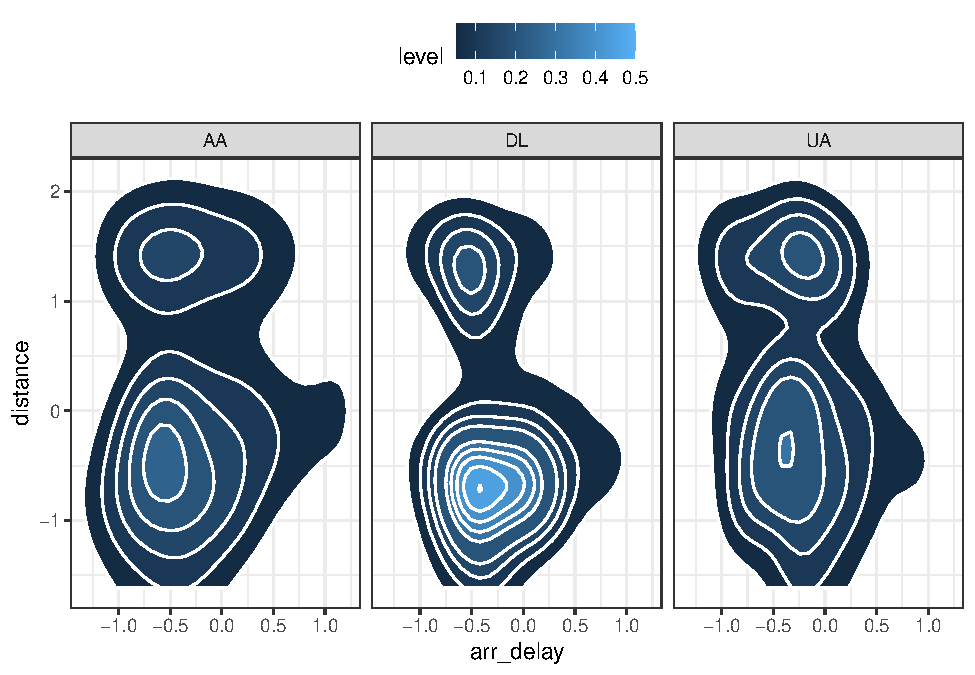
\includegraphics{stat437_HW3_files/figure-latex/unnamed-chunk-5-2.pdf}

\begin{Shaded}
\begin{Highlighting}[]
\FunctionTok{ggplot}\NormalTok{(flights.df) }\SpecialCharTok{+} \FunctionTok{geom\_point}\NormalTok{(}\FunctionTok{aes}\NormalTok{(dep\_delay, arr\_delay, }\AttributeTok{color =}\NormalTok{ kmclus2,}
    \AttributeTok{shape =}\NormalTok{ month)) }\SpecialCharTok{+} \FunctionTok{labs}\NormalTok{(}\AttributeTok{x =} \StringTok{"Departure Delay"}\NormalTok{, }\AttributeTok{y =} \StringTok{"Arrival Delay"}\NormalTok{,}
    \AttributeTok{title =} \StringTok{"K = 2"}\NormalTok{, }\AttributeTok{subtitle =} \StringTok{"Departure Delay vs. Arrival Delay"}\NormalTok{) }\SpecialCharTok{+}
    \FunctionTok{theme\_bw}\NormalTok{()}
\end{Highlighting}
\end{Shaded}

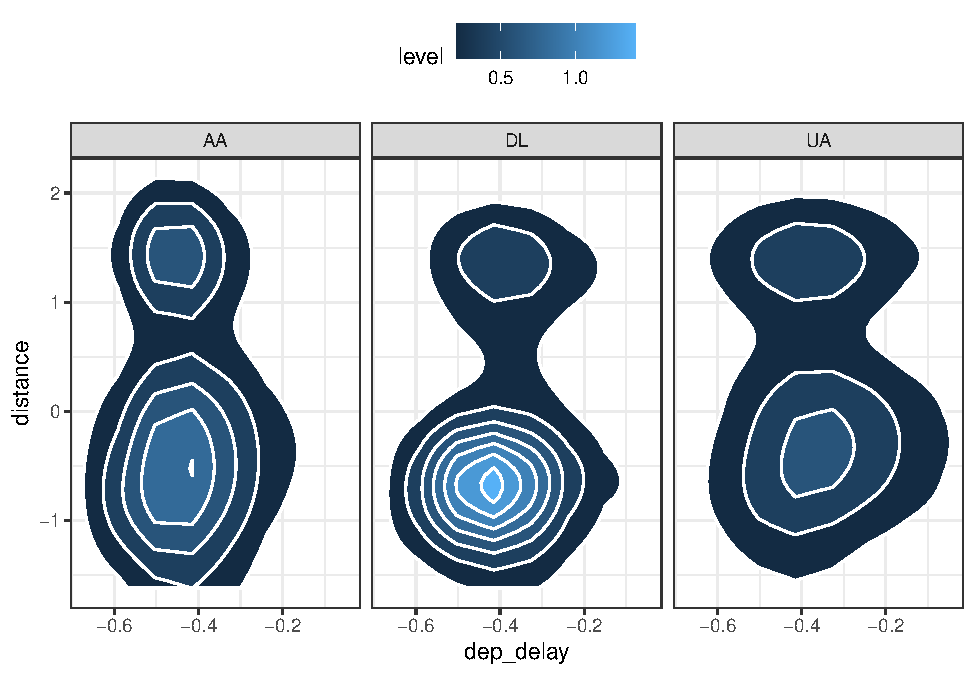
\includegraphics{stat437_HW3_files/figure-latex/unnamed-chunk-5-3.pdf}

\begin{Shaded}
\begin{Highlighting}[]
\FunctionTok{table}\NormalTok{(flights.df}\SpecialCharTok{$}\NormalTok{kmclus2, flights.df}\SpecialCharTok{$}\NormalTok{month)}
\end{Highlighting}
\end{Shaded}

\begin{verbatim}
##    
##        2    7
##   1 7508 8541
##   2 2351 3382
\end{verbatim}

\textbf{K = 3 Visualization}

The results for the k = 3 clustering are similar to the results of the k
= 2 clustering. There is no perceivable trend, and the clusters do not
capture any meaningful pattern in the data. This is unsurprising, given
that no trend appears to exist in the data in the first place. Notably,
the clustering did capture that one group of data, the UA data, tended
to have longer flights both in terms of distance and air time. This is
reflected in the blue clusters.

\begin{Shaded}
\begin{Highlighting}[]
\CommentTok{\# k = 3}
\FunctionTok{ggplot}\NormalTok{(flights.df) }\SpecialCharTok{+} \FunctionTok{geom\_point}\NormalTok{(}\FunctionTok{aes}\NormalTok{(dep\_delay, distance, }\AttributeTok{color =}\NormalTok{ kmclus3,}
    \AttributeTok{shape =}\NormalTok{ carrier)) }\SpecialCharTok{+} \FunctionTok{labs}\NormalTok{(}\AttributeTok{x =} \StringTok{"Departure Delay"}\NormalTok{, }\AttributeTok{y =} \StringTok{"Distance"}\NormalTok{,}
    \AttributeTok{title =} \StringTok{"K = 3"}\NormalTok{, }\AttributeTok{subtitle =} \StringTok{"Departure Delay vs. Distance"}\NormalTok{) }\SpecialCharTok{+}
    \FunctionTok{theme\_bw}\NormalTok{()}
\end{Highlighting}
\end{Shaded}

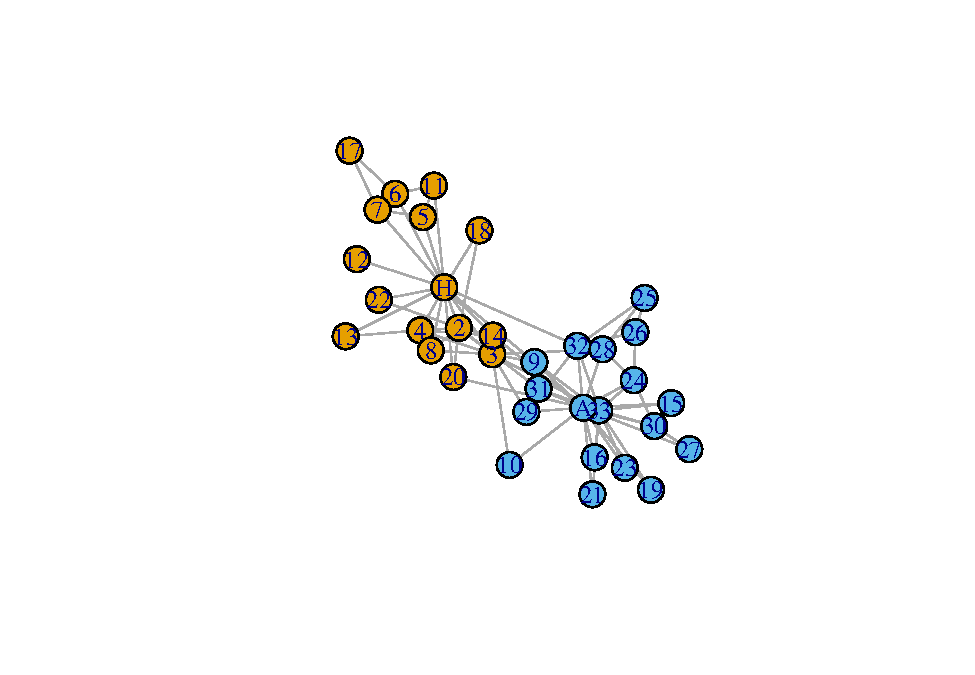
\includegraphics{stat437_HW3_files/figure-latex/unnamed-chunk-6-1.pdf}

\begin{Shaded}
\begin{Highlighting}[]
\FunctionTok{ggplot}\NormalTok{(flights.df) }\SpecialCharTok{+} \FunctionTok{geom\_point}\NormalTok{(}\FunctionTok{aes}\NormalTok{(arr\_delay, air\_time, }\AttributeTok{color =}\NormalTok{ kmclus3,}
    \AttributeTok{shape =}\NormalTok{ carrier)) }\SpecialCharTok{+} \FunctionTok{labs}\NormalTok{(}\AttributeTok{x =} \StringTok{"Arrival Delay"}\NormalTok{, }\AttributeTok{y =} \StringTok{"Air Time"}\NormalTok{,}
    \AttributeTok{title =} \StringTok{"K = 3"}\NormalTok{, }\AttributeTok{subtitle =} \StringTok{"Arrival Delay vs. Air Time"}\NormalTok{) }\SpecialCharTok{+}
    \FunctionTok{theme\_bw}\NormalTok{()}
\end{Highlighting}
\end{Shaded}

\includegraphics{stat437_HW3_files/figure-latex/unnamed-chunk-6-2.pdf}

\begin{Shaded}
\begin{Highlighting}[]
\FunctionTok{ggplot}\NormalTok{(flights.df) }\SpecialCharTok{+} \FunctionTok{geom\_point}\NormalTok{(}\FunctionTok{aes}\NormalTok{(dep\_delay, arr\_delay, }\AttributeTok{color =}\NormalTok{ kmclus3,}
    \AttributeTok{shape =}\NormalTok{ carrier)) }\SpecialCharTok{+} \FunctionTok{labs}\NormalTok{(}\AttributeTok{x =} \StringTok{"Departure Delay"}\NormalTok{, }\AttributeTok{y =} \StringTok{"Arrival Delay"}\NormalTok{,}
    \AttributeTok{title =} \StringTok{"K = 3"}\NormalTok{, }\AttributeTok{subtitle =} \StringTok{"Departure Delay vs. Arrival Delay"}\NormalTok{) }\SpecialCharTok{+}
    \FunctionTok{theme\_bw}\NormalTok{()}
\end{Highlighting}
\end{Shaded}

\includegraphics{stat437_HW3_files/figure-latex/unnamed-chunk-6-3.pdf}

\begin{Shaded}
\begin{Highlighting}[]
\FunctionTok{table}\NormalTok{(flights.df}\SpecialCharTok{$}\NormalTok{kmclus3, flights.df}\SpecialCharTok{$}\NormalTok{carrier)}
\end{Highlighting}
\end{Shaded}

\begin{verbatim}
##    
##       AA   DL   UA
##   1 2887 3365 4247
##   2 1295 2425 1889
##   3  986 1696 2992
\end{verbatim}

\textbf{3.2)} \emph{Use \texttt{set.seed(123)} to randomly extract 50
observations, and to these 50 observations, apply hierarchical
clustering with average linkage. (i) Cut the dendrogram to obtain 3
clusters with leafs annotated by \texttt{carrier} names and resulting
clusters colored distinctly, and report the corresponding height of cut.
(ii) In addition, cut the dendrogram to obtain 2 clusters with leafs
annotated by \texttt{month} numbers and resulting clusters colored
distinctly, and report the corresponding height of cut. Here are some
hints: say, you save the randomly extracted 50 observations into an
object \texttt{ds3sd}, for these observations save their
\texttt{carrier} names by keeping their object type but save
\texttt{month} numbers as a \texttt{character} vector, make sure that
\texttt{ds3sd} is a \texttt{matrix}, transpose \texttt{ds3sd} into
\texttt{tmp}, assign to \texttt{tmp} column names with their
corresponding carrier names or month numbers, and then transpose
\texttt{tmp} and save it as \texttt{ds3sd}; this way, you are done
assigning cluster labels to each observation in \texttt{ds3sd}; then you
are ready to use the commands in the file \texttt{Plotggdendro.r} to
create the desired dendrograms.}

\textbf{i) Dendrogram for k = 3}

The height of the cut to obtain 3 clusters was 2.036.

\begin{Shaded}
\begin{Highlighting}[]
\FunctionTok{library}\NormalTok{(ggdendro)}
\FunctionTok{set.seed}\NormalTok{(}\DecValTok{123}\NormalTok{)}

\CommentTok{\# Subset the data and prepare for ggdendro}
\NormalTok{flights.sample }\OtherTok{\textless{}{-}}\NormalTok{ flights.df[}\FunctionTok{sample}\NormalTok{(}\DecValTok{1}\SpecialCharTok{:}\FunctionTok{nrow}\NormalTok{(flights.df), }\DecValTok{50}\NormalTok{),}
\NormalTok{    ] }\SpecialCharTok{\%\textgreater{}\%}
    \FunctionTok{select}\NormalTok{(}\DecValTok{1}\SpecialCharTok{:}\DecValTok{6}\NormalTok{)}
\NormalTok{carriers }\OtherTok{\textless{}{-}}\NormalTok{ flights.sample}\SpecialCharTok{$}\NormalTok{carrier}
\NormalTok{months }\OtherTok{\textless{}{-}} \FunctionTok{as.character}\NormalTok{(flights.sample}\SpecialCharTok{$}\NormalTok{month)}
\NormalTok{flights.sample }\OtherTok{\textless{}{-}} \FunctionTok{as.matrix}\NormalTok{(flights.sample[}\SpecialCharTok{{-}}\NormalTok{(}\DecValTok{1}\SpecialCharTok{:}\DecValTok{2}\NormalTok{)])}
\NormalTok{tmp }\OtherTok{\textless{}{-}} \FunctionTok{as.data.frame}\NormalTok{(}\FunctionTok{t}\NormalTok{(flights.sample))}

\CommentTok{\# Assign column names to carrier label}
\FunctionTok{colnames}\NormalTok{(tmp) }\OtherTok{\textless{}{-}}\NormalTok{ carriers}
\NormalTok{carriers.sample }\OtherTok{\textless{}{-}} \FunctionTok{t}\NormalTok{(tmp)}

\CommentTok{\# Calculate dissimilarity measure}
\NormalTok{carriers.dissm }\OtherTok{\textless{}{-}} \FunctionTok{dist}\NormalTok{(}\FunctionTok{scale}\NormalTok{(carriers.sample))}

\CommentTok{\# Implement the hierachical clustering}
\NormalTok{hc.avg }\OtherTok{\textless{}{-}} \FunctionTok{hclust}\NormalTok{(carriers.dissm, }\AttributeTok{method =} \StringTok{"average"}\NormalTok{)}
\CommentTok{\# ggdendrogram(hc.avg, rotate = F)}

\FunctionTok{source}\NormalTok{(}\StringTok{"C:/Plotggdendro.r"}\NormalTok{)}
\NormalTok{cutheight }\OtherTok{=}\NormalTok{ hc.avg}\SpecialCharTok{$}\NormalTok{height[}\FunctionTok{length}\NormalTok{(hc.avg}\SpecialCharTok{$}\NormalTok{height) }\SpecialCharTok{{-}} \DecValTok{3}\NormalTok{]}
\NormalTok{droplot }\OtherTok{=} \FunctionTok{plot\_ggdendro}\NormalTok{(}\FunctionTok{dendro\_data\_k}\NormalTok{(hc.avg, }\DecValTok{3}\NormalTok{), }\AttributeTok{direction =} \StringTok{"tb"}\NormalTok{,}
    \AttributeTok{heightReferece =}\NormalTok{ cutheight, }\AttributeTok{expand.y =} \FloatTok{0.2}\NormalTok{)}
\end{Highlighting}
\end{Shaded}

\begin{verbatim}
## Warning: Using `size` aesthetic for lines was deprecated in ggplot2 3.4.0.
## i Please use `linewidth` instead.
## This warning is displayed once every 8 hours.
## Call `lifecycle::last_lifecycle_warnings()` to see where this warning was
## generated.
\end{verbatim}

\begin{Shaded}
\begin{Highlighting}[]
\NormalTok{droplot}
\end{Highlighting}
\end{Shaded}

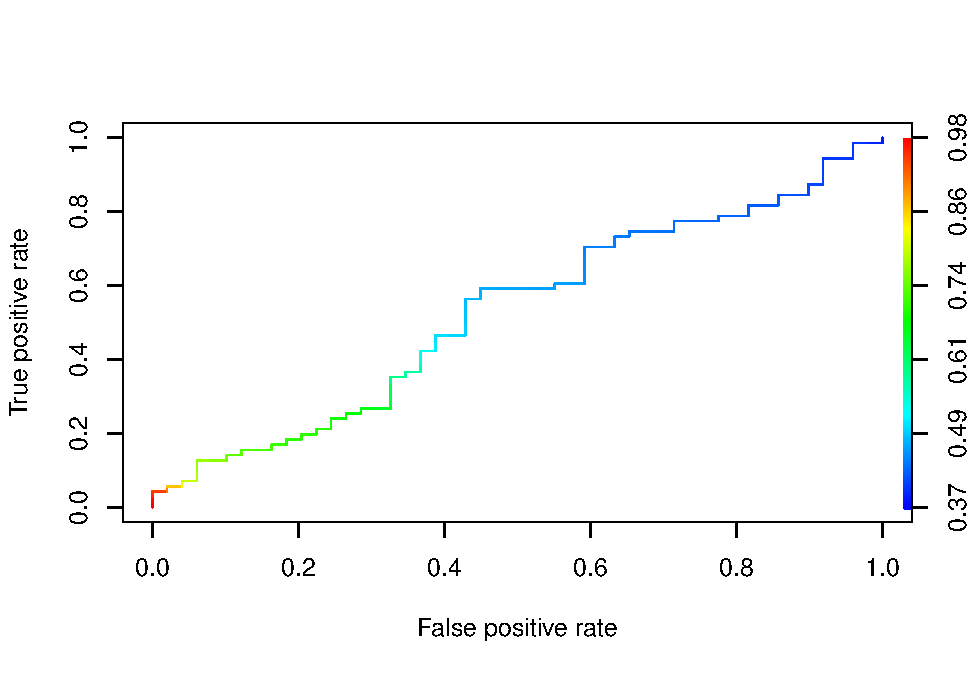
\includegraphics{stat437_HW3_files/figure-latex/unnamed-chunk-7-1.pdf}

\begin{Shaded}
\begin{Highlighting}[]
\FunctionTok{print}\NormalTok{(cutheight)}
\end{Highlighting}
\end{Shaded}

\begin{verbatim}
## [1] 2.036656
\end{verbatim}

\textbf{ii) Dendrogram for k = 2}

The height of cut to obtain 2 clusters was 2.62.

\begin{Shaded}
\begin{Highlighting}[]
\CommentTok{\# Assign column names to month label}
\NormalTok{tmp }\OtherTok{\textless{}{-}} \FunctionTok{as.data.frame}\NormalTok{(}\FunctionTok{t}\NormalTok{(flights.sample))}
\FunctionTok{colnames}\NormalTok{(tmp) }\OtherTok{\textless{}{-}}\NormalTok{ months}
\NormalTok{months.sample }\OtherTok{\textless{}{-}} \FunctionTok{t}\NormalTok{(tmp)}

\CommentTok{\# Calculate dissimilarity measure}
\NormalTok{months.dissm }\OtherTok{\textless{}{-}} \FunctionTok{dist}\NormalTok{(}\FunctionTok{scale}\NormalTok{(months.sample))}

\CommentTok{\# Implement the hierachical clustering}
\NormalTok{hc.avg }\OtherTok{\textless{}{-}} \FunctionTok{hclust}\NormalTok{(months.dissm, }\AttributeTok{method =} \StringTok{"average"}\NormalTok{)}
\CommentTok{\# ggdendrogram(hc.avg, rotate = F)}


\NormalTok{cutheight }\OtherTok{=}\NormalTok{ hc.avg}\SpecialCharTok{$}\NormalTok{height[}\FunctionTok{length}\NormalTok{(hc.avg}\SpecialCharTok{$}\NormalTok{height) }\SpecialCharTok{{-}} \DecValTok{2}\NormalTok{]}
\NormalTok{droplot }\OtherTok{=} \FunctionTok{plot\_ggdendro}\NormalTok{(}\FunctionTok{dendro\_data\_k}\NormalTok{(hc.avg, }\DecValTok{2}\NormalTok{), }\AttributeTok{direction =} \StringTok{"tb"}\NormalTok{,}
    \AttributeTok{heightReferece =}\NormalTok{ cutheight, }\AttributeTok{expand.y =} \FloatTok{0.2}\NormalTok{)}
\NormalTok{droplot}
\end{Highlighting}
\end{Shaded}

\includegraphics{stat437_HW3_files/figure-latex/unnamed-chunk-8-1.pdf}

\begin{Shaded}
\begin{Highlighting}[]
\FunctionTok{print}\NormalTok{(cutheight)}
\end{Highlighting}
\end{Shaded}

\begin{verbatim}
## [1] 2.619144
\end{verbatim}

\end{document}
